\chapter{Вычисления в быстрых системах}

\section{Примеры}

\noindent Рассмотрим $\mathbb{T} = \{2, 3\}$






\subsection{Упрощение}

\noindent От конвейера в 60 требуется отделить 15 и 45:

\vspace{0.1in}

$\frac{15}{60} = \frac{1}{4} = \frac{1}{2}\cdot\frac{1}{2} \ , \ \frac{45}{60} = \frac{3}{4} = 3 \cdot \frac{1}{2}\cdot\frac{1}{2}$

\vspace{0.5in}




\begin{minipage}{0.4\textwidth}
	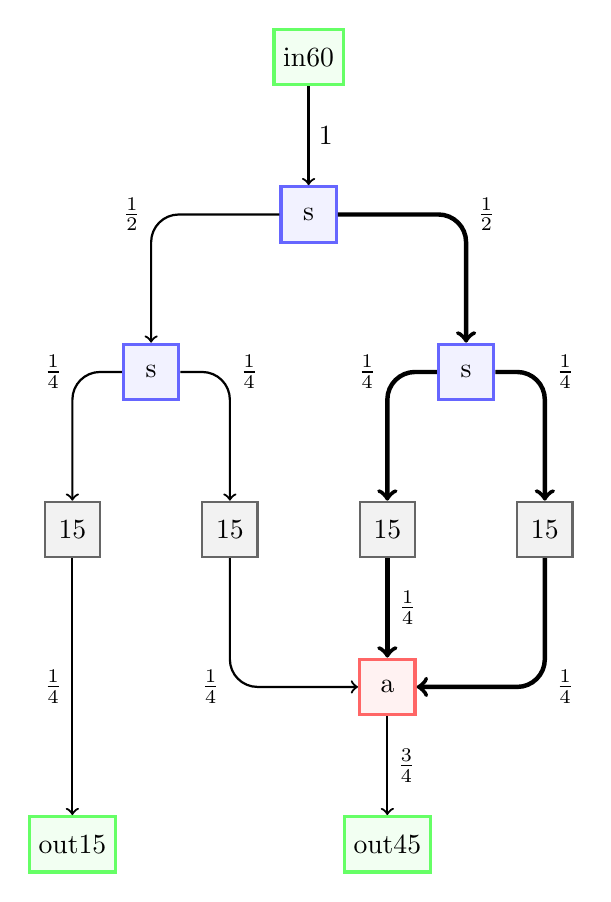
\begin{tikzpicture}[
		s/.style = {rectangle, draw=blue!60, fill=blue!5, very thick, minimum size=20},
		a/.style = {rectangle, draw=red!60, fill=red!5, very thick, minimum size=20},
		o/.style = {rectangle, draw=green!60, fill=green!5, very thick, minimum size=20},
		t/.style = {rectangle, draw=black!60, fill=black!5, thick, minimum size=20},
		r/.style = {->, thick, rounded corners=10pt},
		!/.style = {->, ultra thick, rounded corners=10pt}
		]
		
		%Nodes
		\node[o]	(in)	at	(0, 4)		{in \newline 60};
		\node[s]	(s1)	at	(0, 2)		{s};
		\node[s]	(s2)	at	(-2, 0)		{s};
		\node[s]	(s3)	at	(2, 0)		{s};
		\node[t]	(t1)	at	(-3, -2)	{15};
		\node[t]	(t2)	at	(-1, -2)	{15};
		\node[t]	(t3)	at	(1, -2)		{15};
		\node[t]	(t4)	at	(3, -2)		{15};
		\node[a]	(a)		at	(1, -4)		{a};
		\node[o]	(out1)	at	(-3, -6)	{out \newline 15};
		\node[o]	(out2)	at	(1, -6)		{out \newline 45};
		
		%Lines
		\draw[r]	(in.south) 	to	node[right]	{$1$}			(s1.north);
		\draw[r]	(s1.west)	-|	node[left]	{$\frac{1}{2}$}	(s2.north);
		\draw[!]	(s1.east)	-|	node[right]	{$\frac{1}{2}$}	(s3.north);
		\draw[r]	(s2.west)	-|	node[left]	{$\frac{1}{4}$}	(t1.north);
		\draw[r]	(s2.east)	-|	node[right]	{$\frac{1}{4}$}	(t2.north);
		\draw[!]	(s3.west)	-|	node[left]	{$\frac{1}{4}$}	(t3.north);
		\draw[!]	(s3.east)	-|	node[right]	{$\frac{1}{4}$}	(t4.north);
		\draw[r]	(t1.south)	to	node[left]	{$\frac{1}{4}$}	(out1.north);
		\draw[r]	(t2.south)	|-	node[left]	{$\frac{1}{4}$}	(a.west);
		\draw[!]	(t3.south)	to	node[right]	{$\frac{1}{4}$}	(a.north);
		\draw[!]	(t4.south)	|-	node[right]	{$\frac{1}{4}$}	(a.east);
		\draw[r]	(a.south)	to	node[right]	{$\frac{3}{4}$}	(out2.north);
	\end{tikzpicture}
	
	\
	
	$$\text{Рис. 1}$$
\end{minipage}
\hspace{37.5pt}
\begin{minipage}{0.1\textwidth}
	$$\equiv$$
\end{minipage}
\hspace{12.5pt}
\begin{minipage}{0.2\textwidth}
	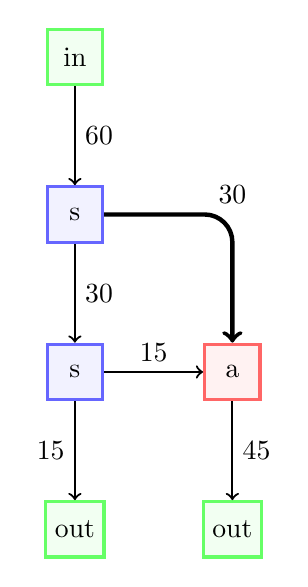
\begin{tikzpicture}[
		s/.style = {rectangle, draw=blue!60, fill=blue!5, very thick, minimum size=20},
		a/.style = {rectangle, draw=red!60, fill=red!5, very thick, minimum size=20},
		o/.style = {rectangle, draw=green!60, fill=green!5, very thick, minimum size=20},
		r/.style = {->, thick, rounded corners=10pt},
		!/.style = {->, ultra thick, rounded corners=10pt}
		]
		
		%Nodes
		\node[o]	(in)	at	(0, 4)	{in};
		\node[s]	(s1)	at	(0, 2)	{s};
		\node[s]	(s2)	at	(0, 0)	{s};
		\node[a]	(a)		at	(2, 0)	{a};
		\node[o]	(out1)	at	(0, -2)	{out};
		\node[o]	(out2)	at	(2, -2)	{out};
		
		%Lines
		\draw[r]	(in.south) 	to	node[right]	{$60$}	(s1.north);
		\draw[r]	(s1.south)	to	node[right]	{$30$}	(s2.north);
		\draw[!]	(s1.east)	-|	node[above]	{$30$}	(a.north);
		\draw[r]	(s2.east)	to	node[above]	{$15$}	(a.west);
		\draw[r]	(s2.south)	to	node[left]	{$15$}	(out1.north);
		\draw[r]	(a.south)	to	node[right]	{$45$}	(out2.north);
	\end{tikzpicture}
	
	\
	
	$$\text{Рис. 2}$$
\end{minipage}

\vspace{0.3in}

Заметим, что на рис. 1 имеется \textbf{область}, в которой разделение безсмысленно, ведь отделённые друг от друга конвейеры затем вновь соединяются. Тогда можно убрать данный разделитель, оставив целиковый \textbf{конвейер}.




\vspace{0.3in}

Для рассмотрения алгебраической картины данной задачи, нам потребуется ввести обозначение: за ответвления в стороны, с припиской в виде числа будем обозначать, что столько-то конвейеров уходят в новую ветку схемы:


\begin{minipage}{0.2\textwidth}
	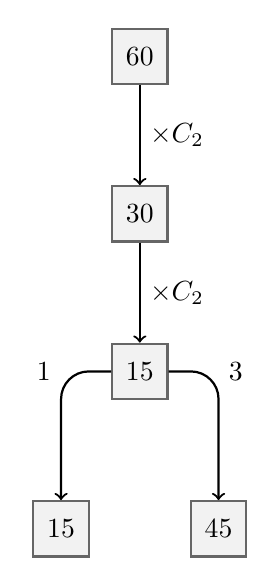
\begin{tikzpicture}[
		t/.style = {rectangle, draw=black!60, fill=black!5, thick, minimum size=20},
		r/.style = {->, thick, rounded corners=10pt}
		]
		
		%Nodes
		\node[t]	(1)		at	(0, 4)		{$60$};
		\node[t]	(2)		at	(0, 2)		{$30$};
		\node[t]	(e)		at	(0, 0)		{$15$};
		\node[t]	(out1)	at	(-1, -2)	{$15$};
		\node[t]	(out2)	at	(1, -2)		{$45$};
		
		%Lines
		\draw[r]	(1.south)	to	node[right]	{$\times C_2$}	(2.north);
		\draw[r]	(2.south)	to	node[right]	{$\times C_2$}	(e.north);
		\draw[r]	(e.west)	-|	node[left]	{$1$}			(out1.north);
		\draw[r]	(e.east)	-|	node[right]	{$3$}			(out2.north);
	\end{tikzpicture}
\end{minipage}
\begin{minipage}{0.1\textwidth}
	$$\equiv$$
\end{minipage}
\begin{minipage}{0.2\textwidth}
	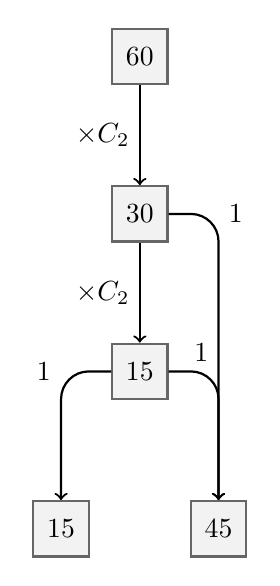
\begin{tikzpicture}[
		t/.style = {rectangle, draw=black!60, fill=black!5, thick, minimum size=20},
		r/.style = {->, thick, rounded corners=10pt}
		]
		
		%Nodes
		\node[t]	(1)		at	(0, 4)		{$60$};
		\node[t]	(2)		at	(0, 2)		{$30$};
		\node[t]	(4)		at	(0, 0)		{$15$};
		\node[t]	(out1)	at	(-1, -2)	{$15$};
		\node[t]	(out2)	at	(1, -2)		{$45$};
		
		%Lines
		\draw[r]	(1.south)	to	node[left]	{$\times C_2$}	(2.north);
		\draw[r]	(2.south)	to	node[left]	{$\times C_2$}	(4.north);
		\draw[r]	(4.west)	-|	node[left]	{$1$}			(out1.north);
		\draw[r]	(2.east)	-|	node[right]	{$1$}			(out2.north);
		\draw[r]	(4.east)	-|	node[above left]	{$1$}		(out2.north);
	\end{tikzpicture}
\end{minipage}

\vspace{0.3in}

Как видим, при упрощении схемы мы получим, что число конвейеров, идущих на соединение не превышает период циклической группы последнего сплиттера: это будет важным моментом, когда мы будем писать программное решение к задаче.
















\vspace{0.5in}

\subsection{Рекурсия}

\noindent От конвейера в 60 требуется отделить 12

\vspace{0.1in}

$\frac{12}{60} = \frac{1}{5} = \frac{1}{6} - \frac{1}{6} = \frac{1}{2}\cdot\frac{1}{3} - \frac{1}{2}\cdot\frac{1}{3} \ , \ \frac{60-12}{60} = \frac{48}{60} = \frac{4}{5} = \frac{4}{6} - \frac{1}{6} = \frac{2}{3} - \frac{1}{2}\cdot\frac{1}{3}$

\vspace{0.5in}

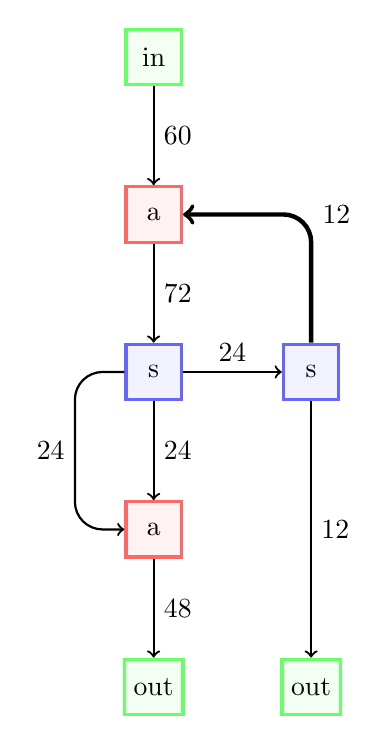
\begin{tikzpicture}[
	s/.style = {rectangle, draw=blue!60, fill=blue!5, very thick, minimum size=20},
	a/.style = {rectangle, draw=red!60, fill=red!5, very thick, minimum size=20},
	o/.style = {rectangle, draw=green!60, fill=green!5, very thick, minimum size=20},
	r/.style = {->, thick, rounded corners=10pt},
	!/.style = {->, ultra thick, rounded corners=10pt}
	]
	
	%Nodes
	\node[o]	(in)	at	(0, 4)	{in};
	\node[a]	(a1)	at	(0, 2)	{a};
	\node[s]	(s1)	at	(0, 0)	{s};
	\node[s]	(s2)	at	(2, 0)	{s};
	\node[a]	(a2)	at	(0, -2)	{a};
	\node[o]	(out1)	at	(0, -4)	{out};
	\node[o]	(out2)	at	(2, -4)	{out};
	
	%Lines
	\draw[r]	(in.south) 	to			node[right]	{$60$}	(a1.north);
	\draw[r]	(a1.south)	to			node[right]	{$72$}	(s1.north);
	\draw[r]	(s1.east)	to			node[above]	{$24$}	(s2.west);
	\draw[!]	(s2.north)	|-			node[right]	{$12$}	(a1.east);
	\draw[r]	(s1.west)	-| (-1, -1) node[left]	{$24$} |- (a2.west);
	\draw[r]	(s1.south)	to			node[right]	{$24$}	(a2.north);
	\draw[r]	(a2.south)	to			node[right]	{$48$}	(out1.north);
	\draw[r]	(s2.south)	to			node[right]	{$12$}	(out2.north);
\end{tikzpicture}

\vspace{0.3in}

% После соединителя представленна схема отделения $\frac16$, которая возвращается себе в зад. На вход всей системе поступает 60 рес/мин, тогда если предположить, что на один круг по этой схеме уходит ровно минута -- то к началу успеют прийти $\frac{60}{6}=10$ ресурсов, и после соединителя пойдёт уже 70 рес/мин. Ещё минуту спустя, на начало прийдёт уже $\frac{70}{6} \approx 11.667$ рес/мин, и после разделителя пойдёт 71.667 рес/мин. Спустя бесконечно долгое время, на участке после разделителя стабилизируется значение в 72 рес/мин. Наконец, отделив от 72, $\frac16$ -- получим требуемые 12, и на остаток 48.

Пускай, в систему импульсами подаётся по одному ресурсу раз в некоторое время%
\footnote{Такая аппроксимация возможна в связи с тем, что конвейер имеет большую скорость, и ресурсы внутри системы друг с другом не взаимодействуют},
тогда внутри делителя на 6 у каждого ресурса будет 6 различных выходов. Положим, первые 5 ресурсов ушли на свои 5 выходов, и как-то распределились в дальнейшей части конструкции. Тогда они поменяли данные, хранящиеся в памяти делителей таким образом, что 6-ой ресурс может уйти только на 6-ой выход. Но этот выход возвращён в начало системы, и тогда 6-ой ресурс становится 1-ым, так как все настройки делителей сбросились%
\footnote{Данная система является примером группы $C_2 \times C_3 = C_6$, в которой 6-ой элемент является и 0-ым}.
Таким образом, данный ресурс снова уходит на один из 5-ти допустимых выходов. Притом получается так, что порядок выходов одинаков, так что данная система является равносильной делителю на 5.



\vspace{0.3in}

\noindent Рассмотрим же теперь алгебраическую картину данной задачи:

\vspace{0.3in}


\begin{minipage}{0.2\textwidth}
	\begin{tikzpicture}[
		t/.style = {rectangle, draw=black!60, fill=black!5, thick, minimum size=20},
		r/.style = {->, thick, rounded corners=10pt}
		]
		
		%Nodes
		\node[t]	(1)		at	(0, 4)		{$60$};
		\node[t]	(3)		at	(0, 2)		{$20$};
		\node[t]	(6)		at	(0, 0)		{$10$};
		\node[t]	(5)		at	(0, -2)		{$12$};
		\node[t]	(out1)	at	(-1, -4)	{$12$};
		\node[t]	(out2)	at	(1, -4)		{$48$};
		
		%Lines
		\draw[r]	(1.south)	to	node[right]	{$\times C_3$}	(2.north);
		\draw[r]	(3.south)	to	node[right]	{$\times C_2$}	(6.north);
		\draw[r]	(6.south)	to	node[right]	{$- \frac{1}{6}$}	(5.north);
		\draw[r]	(5.west)	-|	node[left]	{$1$}			(out1.north);
		\draw[r]	(5.east)	-|	node[right]	{$4$}			(out2.north);
	\end{tikzpicture}
\end{minipage}
\begin{minipage}{0.1\textwidth}
	$$\equiv$$
\end{minipage}
\begin{minipage}{0.2\textwidth}
	\begin{tikzpicture}[
		t/.style = {rectangle, draw=black!60, fill=black!5, thick, minimum size=20},
		r/.style = {->, thick, rounded corners=10pt}
		]
		
		%Nodes
		\node[t]	(1)		at	(0, 4)		{$60$};
		\node[t]	(3)		at	(0, 2)		{$20$};
		\node[t]	(6)		at	(0, 0)		{$10$};
		\node[t]	(5)		at	(0, -2)		{$12$};
		\node[t]	(out2)	at	(1, -2)		{$48$};
		
		%Lines
		\draw[r]	(1.south)	to	node[right]	{$\times C_3$}	(2.north);
		\draw[r]	(3.south)	to	node[left]	{$\times C_2$}	(6.north);
		\draw[r]	(6.south)	to	node[left]	{$- \frac{1}{6}$}	(5.north);
		\draw[r]	(3.east)	-|	node[right]	{$2$}			(out2.north);
	\end{tikzpicture}
\end{minipage}

\vspace{0.3in}

Забавно, что граф можнт разбиваться на несколько, казалось бы независимых ветвей, но применив операцию возврата в одной ветви -- автоматически меняется значение и во всех других ветвях. 












\vspace{0.5in}

\subsection{Вариативность}

\noindent От конвейера в 60 требуется отделить 6. Рассмотрим все (сокращённые) варианты такой схемы:

$\frac{6}{60} = \frac{1}{10} = \frac{1}{12} - \frac{2}{12} = \frac{1}{2}\cdot\frac{1}{2}\cdot\frac{1}{3} - \frac{1}{6}$

\vspace{0.5in}



\begin{minipage}{0.2\textwidth}
	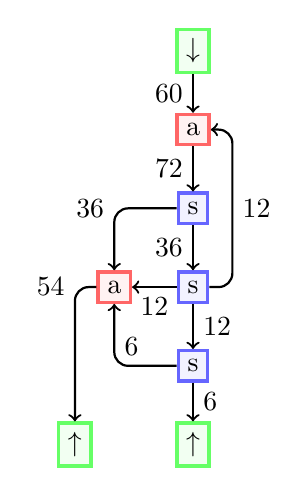
\begin{tikzpicture}[
		s/.style = {rectangle, draw=blue!60,	fill=blue!5,	very thick, minimum size=10},
		a/.style = {rectangle, draw=red!60,		fill=red!5,		very thick, minimum size=10},
		o/.style = {rectangle, draw=green!60,	fill=green!5,	very thick, minimum size=10},
		r/.style = {->, thick, rounded corners=5pt}
		]
		
		%Nodes
		\node[o]	(in)	at	(0, 3)		{$\downarrow$};
		\node[a]	(a1)	at	(0, 2)		{a};
		\node[s]	(s1)	at	(0, 1)		{s};
		\node[s]	(s2)	at	(0, 0)		{s};
		\node[s]	(s3)	at	(0, -1)		{s};
		\node[a]	(a2)	at	(-1, 0)		{a};
		\node[o]	(out1)	at	(-1.5, -2)		{$\uparrow$};
		\node[o]	(out2)	at	(0, -2)	{$\uparrow$};
		
		%Lines
		\draw[r]	(in.south)	to	node[left]	{$60$}	(a1.north);
		\draw[r]	(a1.south)	to	node[left]	{$72$}	(s1.north);
		\draw[r]	(s1.south)	to	node[left]	{$36$}	(s2.north);
		\draw[r]	(s2.east)	-| (0.5, 1) node[right] {$12$} |- (a1.east);
		\draw[r]	(s2.south)	to	node[right]	{$12$}	(s3.north);
		\draw[r]	(s1.west)	-|	node[left]	{$36$}	(a2.north);
		\draw[r]	(s2.west)	to	node[below]	{$12$}	(a2.east);
		\draw[r]	(s3.west)	-|	node[above right]	{$6$}	(a2.south);
		\draw[r]	(a2.west)	-|	node[left]	{$54$}	(out1.north);
		\draw[r]	(s3.south)	to	node[right]	{$6$}	(out2.north);
	\end{tikzpicture}
	
	\
	
	$$\text{Рис. 1}$$
\end{minipage}
\hspace{15pt}
\begin{minipage}{0.2\textwidth}
	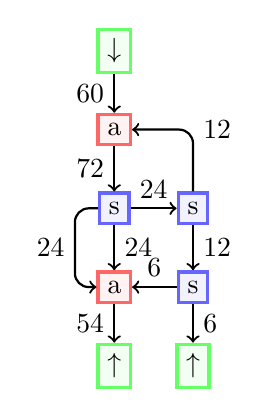
\begin{tikzpicture}[
		s/.style = {rectangle, draw=blue!60,	fill=blue!5,	very thick, minimum size=10},
		a/.style = {rectangle, draw=red!60,		fill=red!5,		very thick, minimum size=10},
		o/.style = {rectangle, draw=green!60,	fill=green!5,	very thick, minimum size=10},
		r/.style = {->, thick, rounded corners=5pt}
		]
		
		%Nodes
		\node[o]	(in)	at	(0, 3)	{$\downarrow$};
		\node[a]	(a1)	at	(0, 2)	{a};
		\node[s]	(s1)	at	(0, 1)	{s};
		\node[a]	(a2)	at	(0, 0)	{a};
		\node[s]	(s2)	at	(1, 1)	{s};
		\node[s]	(s3)	at	(1, 0)	{s};
		\node[o]	(out1)	at	(0, -1)	{$\uparrow$};
		\node[o]	(out2)	at	(1, -1)	{$\uparrow$};
		
		%Lines
		\draw[r]	(in.south)	to	node[left]	{$60$}	(a1.north);
		\draw[r]	(a1.south)	to	node[left]	{$72$}	(s1.north);
		\draw[r]	(s1.east)	to	node[above]	{$24$}	(s2.west);
		\draw[r]	(s2.north)	|-	node[right]	{$12$}	(a1.east);
		\draw[r]	(s2.south)	to	node[right]	{$12$}	(s3.north);
		\draw[r]	(s1.south)	to	node[right]	{$24$}	(a2.north);
		\draw[r]	(s1.west)	-| (-0.5, 0.5) node[left] {$24$} |- (a2.west);
		\draw[r]	(s3.west)	to	node[above]	{$6$}	(a2.east);
		\draw[r]	(a2.south)	to	node[left]	{$54$}	(out1.north);
		\draw[r]	(s3.south)	to	node[right]	{$6$}	(out2.north);
	\end{tikzpicture}
	
	\
	
	$$\text{Рис. 2}$$
\end{minipage}
\hspace{15pt}
\begin{minipage}{0.2\textwidth}
	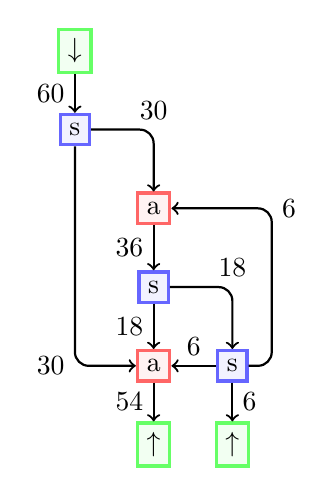
\begin{tikzpicture}[
		s/.style = {rectangle, draw=blue!60,	fill=blue!5,	very thick, minimum size=10},
		a/.style = {rectangle, draw=red!60,		fill=red!5,		very thick, minimum size=10},
		o/.style = {rectangle, draw=green!60,	fill=green!5,	very thick, minimum size=10},
		r/.style = {->, thick, rounded corners=5pt}
		]
		
		%Nodes
		\node[o]	(in)	at	(0, 3)		{$\downarrow$};
		\node[s]	(s1)	at	(0, 2)		{s};
		\node[a] 	(a1)	at	(1, 1)		{a};
		\node[s]	(s2)	at	(1, 0)		{s};
		\node[s]	(s3)	at	(2, -1)		{s};
		\node[a]	(a2)	at	(1, -1)		{a};
		\node[o]	(out1)	at	(1, -2)		{$\uparrow$};
		\node[o]	(out2)	at	(2, -2)		{$\uparrow$};
		
		%Lines
		\draw[r]	(in.south)	to	node[left]	{$60$}	(s1.north);
		\draw[r]	(s1.east)	-|	node[above]	{$30$}	(a1.north);
		\draw[r]	(a1.south)	to	node[left]	{$36$}	(s2.north);
		\draw[r]	(s2.east)	-|	node[above]	{$18$}	(s3.north);
		\draw[r]	(s1.south)	|-	node[left]	{$30$}	(a2.west);
		\draw[r]	(s2.south)	to	node[left]	{$18$}	(a2.north);
		\draw[r]	(s3.west)	to	node[above]	{$6$}	(a2.east);
		\draw[r]	(a2.south)	to	node[left]	{$54$}	(out1.north);
		\draw[r]	(s3.south)	to	node[right]	{$6$}	(out2.north);
		\draw[r]	(s3.east)	to (2.5, -1) |- node[right] {$6$} (a1.east);
	\end{tikzpicture}
	
	\
	
	$$\text{Рис. 3}$$
\end{minipage}
\hspace{15pt}
\begin{minipage}{0.2\textwidth}
	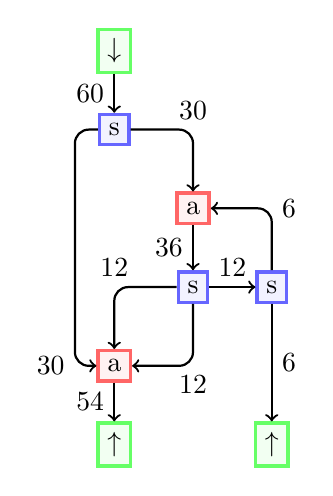
\begin{tikzpicture}[
		s/.style = {rectangle, draw=blue!60,	fill=blue!5,	very thick, minimum size=10},
		a/.style = {rectangle, draw=red!60,		fill=red!5,		very thick, minimum size=10},
		o/.style = {rectangle, draw=green!60,	fill=green!5,	very thick, minimum size=10},
		r/.style = {->, thick, rounded corners=5pt}
		]
		
		%Nodes
		\node[o]	(in)	at	(0, 3)		{$\downarrow$};
		\node[s]	(s1)	at	(0, 2)		{s};
		\node[a] 	(a1)	at	(1, 1)		{a};
		\node[s]	(s2)	at	(1, 0)		{s};
		\node[s]	(s3)	at	(2, 0)		{s};
		\node[a]	(a2)	at	(0, -1)		{a};
		\node[o]	(out1)	at	(0, -2)		{$\uparrow$};
		\node[o]	(out2)	at	(2, -2)		{$\uparrow$};
		
		%Lines
		\draw[r]	(in.south)	to	node[left]	{$60$}	(s1.north);
		\draw[r]	(s1.east)	-|	node[above]	{$30$}	(a1.north);
		\draw[r]	(a1.south)	to	node[left]	{$36$}	(s2.north);
		\draw[r]	(s2.east)	to	node[above]	{$12$}	(s3.west);
		\draw[r]	(s1.west)	to (-0.5, 2) |-	node[left]	{$30$}	(a2.west);
		\draw[r]	(s2.south)	|-	node[below]	{$12$}	(a2.east);
		\draw[r]	(s2.west)	-|	node[above]	{$12$}	(a2.north);
		\draw[r]	(a2.south)	to	node[left]	{$54$}	(out1.north);
		\draw[r]	(s3.south)	to	node[right]	{$6$}	(out2.north);
		\draw[r]	(s3.north)	|- 	node[right] {$6$}	(a1.east);
	\end{tikzpicture}
	
	\
	
	$$\text{Рис. 4}$$
\end{minipage}



\vspace{0.3in}

Заметим, что в во всех схемах, являющихся сокращёнными вариациями реализации одного и того же решения, число соединителей и разъединителей -- инвариантно относительно топологии графа. Притом сохраняется ещё и число входов/выходов конкретного узла, а так же сохраняются подструктуры по типу циклов:





\vspace{0.5in}

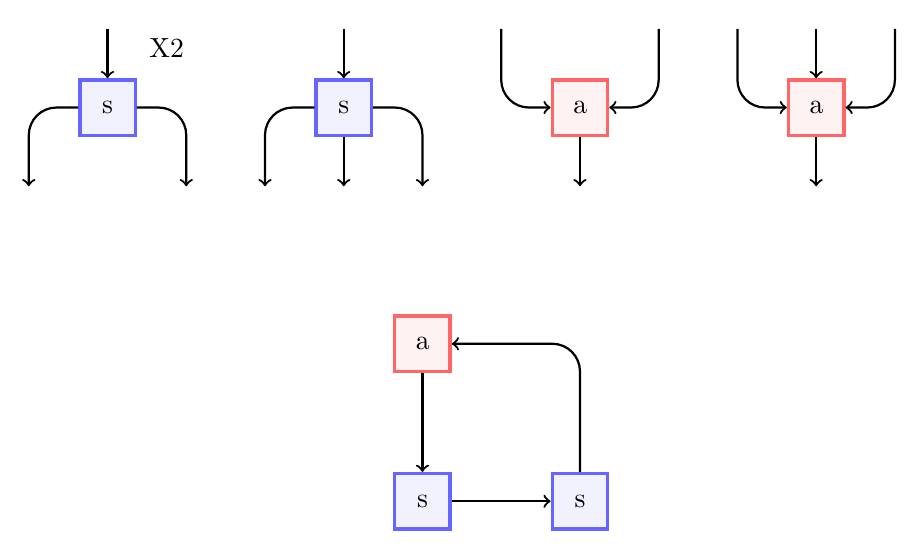
\begin{tikzpicture}[
		s/.style = {rectangle, draw=blue!60,	fill=blue!5,	very thick, minimum size=20},
		a/.style = {rectangle, draw=red!60,		fill=red!5,		very thick, minimum size=20},
		o/.style = {rectangle, draw=green!60,	fill=green!5,	very thick, minimum size=20},
		r/.style = {->, thick, rounded corners=10pt}
		]
		
		\node[s]	(s1)	at	(-6, 0)		{s};
		\draw[r]	(-6, 1)	to	(s1.north);
		\draw[r]	(s1.west)	-|	(-7, -1);
		\draw[r]	(s1.east)	-|	(-5, -1);
		\node (x) at (-5.25, 0.75) {X2};
		
		\node[s]	(s2)	at	(-3, 0)		{s};
		\draw[r]	(-3, 1)		to	(s2.north);
		\draw[r]	(s2.west)	-|	(-4, -1);
		\draw[r]	(s2.east)	-|	(-2, -1);
		\draw[r]	(s2.south)	to	(-3, -1);
		
		\node[a]	(a1)	at	(0, 0)		{a};
		\draw[r]	(-1, 1)		|-	(a1.west);
		\draw[r]	(1, 1)		|-	(a1.east);
		\draw[r]	(a1.south)	to	(0, -1);
		
		\node[a]	(a2)	at	(3, 0)		{a};
		\draw[r]	(2, 1)		|-	(a2.west);
		\draw[r]	(4, 1)		|-	(a2.east);
		\draw[r]	(3, 1)		to	(a2.north);
		\draw[r]	(a2.south)	to	(3, -1);
		
		
		
		\node[a]	(a3)	at	(-2, -3)	{a};
		\node[s]	(s4)	at	(-2, -5)	{s};
		\node[s]	(s5)	at	(0, -5)		{s};	
		\draw[r]	(a3.south)	to	(s4.north);
		\draw[r]	(s4.east)	to	(s5.west);
		\draw[r]	(s5.north)	|-	(a3.east);		
\end{tikzpicture}



\vspace{0.5in}

Так же важно помнить, что это всё было только одно решерние: $s = 12$, а ведь можно было взять первые пару ближайших стандартных чисел $(12, 16, 18, \ldots)$, или стандартные числа, являющиеся чисто степенями $(16, 32, 27, \ldots)$. Так же в решении можно было использоавть нетривиальные разложения по типу: $\frac56 = \frac12 + \frac13$



\vspace{0.3in}

















\vspace{0.5in}

\subsection{Большие схемы}

\noindent Рассмотрим схему побольше: отделить $\frac17$, $\frac15$ и $\frac13$ одновременно от одного конвейера.

$\text{lcm}(3, 5, 7) = 105$

\begin{align*}
	&\frac{1}{7} = \frac{15}{105} = \frac{15}{2^2 3^3} - \frac{3}{108} = \frac{5}{36} - \frac{1}{36} = \frac{1}{36} + \frac{1}{9} - \frac{1}{36} \\
	&\frac{1}{5} = \frac{21}{105} = \frac{21}{2^2 3^3} - \frac{3}{108} = \frac{7}{36} - \frac{1}{36} = \frac{1}{36} + \frac{1}{6} - \frac{1}{36} \\
	&\frac{1}{3} = \frac{35}{105} = \frac{35}{2^2 3^3} - \frac{3}{108} = \frac{1}{36} + \frac{2}{27} + \frac{2}{9} - \frac{1}{36}
\end{align*}

Остаток: $\frac{34}{105}$






\vspace{0.5in}


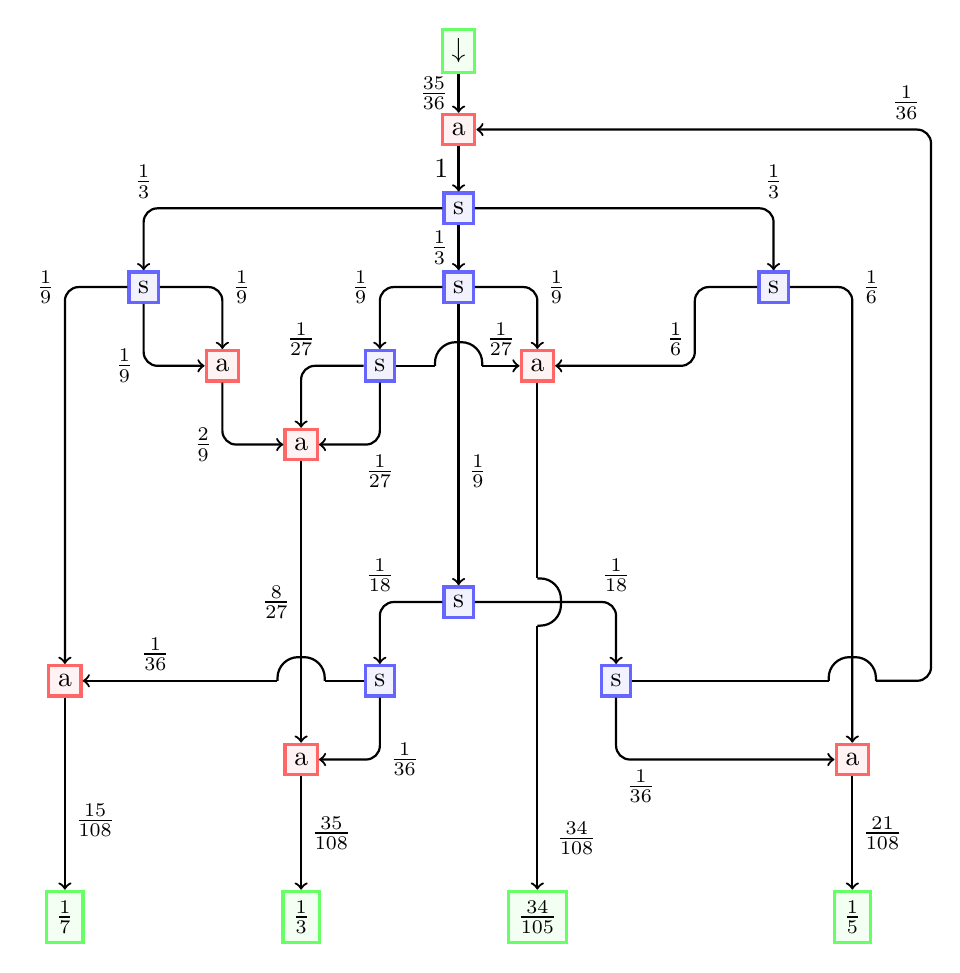
\begin{tikzpicture}[
	s/.style = {rectangle, draw=blue!60,	fill=blue!5,	very thick, minimum size=10},
	a/.style = {rectangle, draw=red!60,		fill=red!5,		very thick, minimum size=10},
	o/.style = {rectangle, draw=green!60,	fill=green!5,	very thick, minimum size=10},
	r/.style = {->, thick, rounded corners=5pt}
	]
	
	%Nodes
	\node[o]	(in)	at	(0, 5)		{$\downarrow$};
	\node[a]	(a1)	at	(0, 4)		{a};
	\node[s]	(s1)	at	(0, 3)		{s};
	
	\node[s]	(s2-l)	at	(-4, 2)		{s};
	\node[s]	(s2-c)	at	(0, 2)		{s};
	\node[s]	(s2-r)	at	(4, 2)		{s};
	\node[a]	(a2-l)	at	(-3, 1)		{a};
	\node[a]	(a2-c)	at	(-2, 0)		{a};
	\node[s]	(s2-2)	at	(-1, 1)		{s};
	\node[a]	(a2-r)	at	(1, 1)		{a};
	
	\node[s]	(s3)	at	(0, -2)		{s};
	\node[s]	(s4-l)	at	(-1, -3)	{s};
	\node[s]	(s4-r)	at	(2, -3)		{s};
	\node[a]	(a3-l)	at	(-5, -3)	{a};
	\node[a]	(a3-c)	at	(-2, -4)	{a};
	\node[a]	(a3-r)	at	(5, -4)		{a};
	
	\node[o]	(out1)	at	(-5, -6)	{$\frac{1}{7}$};
	\node[o]	(out2)	at	(-2, -6)	{$\frac{1}{3}$};
	\node[o]	(out3)	at	(1, -6)		{$\frac{34}{105}$};
	\node[o]	(out4)	at	(5, -6)		{$\frac{1}{5}$};
	
	
	
	%Lines
	\draw[r]	(in.south)		to	node[left]			{$\frac{35}{36}$}	(a1.north);
	\draw[r]	(a1.south)		to	node[left]			{$1$}				(s1.north);
	\draw[r]	(s1.west)		-|	node[above]			{$\frac13$}			(s2-l.north);
	\draw[r]	(s1.south)		to	node[left]			{$\frac13$}			(s2-c.north);
	\draw[r]	(s1.east)		-|	node[above]			{$\frac13$}			(s2-r.north);
	
	\draw[r]	(s2-l.south)	|-	node[left]			{$\frac19$}			(a2-l.west);
	\draw[r]	(s2-l.east)		-|	node[right]			{$\frac19$}			(a2-l.north);
	\draw[r]	(s2-c.west)		-|	node[left]			{$\frac19$}			(s2-2.north);
	\draw[r]	(s2-2.west)		-|	node[above]			{$\frac1{27}$}		(a2-c.north);
	\draw[r]	(s2-2.south)	|-	node[below]			{$\frac1{27}$}		(a2-c.east);
	\draw[r]	(a2-l.south)	|-	node[left]			{$\frac29$}			(a2-c.west);
	\draw[r]	(s2-c.east)		-|	node[right]			{$\frac19$}			(a2-r.north);
	
	\draw[r] (s2-r.west) to (3, 2) |- node[above left] {$\frac16$} (a2-r.east);
	\draw[thick] (s2-2.east) -- (-0.3, 1);
	\draw[thick, rounded corners=7.5pt] (-0.3, 1) |- (0, 1.3);
	\draw[thick, rounded corners=7.5pt] (0, 1.3) -| (0.3, 1);
	\draw[r] (0.3, 1) to node[above] {$\frac{1}{27}$} (a2-r.west);
	
	\draw[r]	(s2-c.south)	to	node[below right]	{$\frac{1}{9}$}		(s3.north);
	\draw[r]	(s3.west)		-|	node[above]			{$\frac{1}{18}$}	(s4-l.north);
	\draw[r]	(s3.east)		-|	node[above]			{$\frac{1}{18}$}	(s4-r.north);
	\draw[r]	(s4-l.south)	|-	node[right]			{$\frac{1}{36}$}	(a3-c.east);
	\draw[r]	(a2-c.south)	to	node[left]			{$\frac{8}{27}$}	(a3-c.north);
	\draw[r]	(s4-r.south)	|-	node[below right]	{$\frac{1}{36}$}	(a3-r.west);
	\draw[r]	(s2-r.east)		-|	node[right]			{$\frac16$}			(a3-r.north);
	\draw[r]	(s2-l.west)		-|	node[left]			{$\frac19$}			(a3-l.north);
	
	\draw[r]	(a3-l.south)	to	node[below right]	{$\frac{15}{108}$}		(out1.north);
	\draw[r]	(a3-c.south)	to	node[right]			{$\frac{35}{108}$}	(out2.north);
	\draw[r]	(a3-r.south)	to	node[right]			{$\frac{21}{108}$}		(out4.north);
	\node (n1) at (1.5, -5) {$\frac{34}{108}$};
	
	\draw[thick] (a2-r.south) -- (1, -1.7);
	\draw[thick, rounded corners=7.5pt] (1, -1.7) -| (1.3, -2);
	\draw[thick, rounded corners=7.5pt] (1.3, -2) |- (1, -2.3);
	\draw[r] (1, -2.3) to (out3.north);
	
	\draw[thick] (s4-r.east) -- (4.7, -3);
	\draw[thick, rounded corners=7.5pt] (4.7, -3) |- (5, -2.7);
	\draw[thick, rounded corners=7.5pt] (5, -2.7) -| (5.3, -3);
	\draw[r] (5.3, -3) to (6, -3) |- node[above left] {$\frac1{36}$} (a1.east);
	
	\draw[thick] (s4-l.west) -- (-1.7, -3);
	\draw[thick, rounded corners=7.5pt] (-1.7, -3) |- (-2, -2.7);
	\draw[thick, rounded corners=7.5pt] (-2, -2.7) -| (-2.3, -3);
	\draw[r] (-2.3, -3) to node[above left] {$\frac1{36}$} (a3-l.east);
	
	
	
\end{tikzpicture}











\vspace{0.5in}

Как мы можем заметить, на схемах побольше появляются две интересные вещи: \\ \underline{пересечеиния конвейеров}%
\footnote{Смотреть приложение \ref{appendix:a}: проблема перекрёстков (brick factory problem)}
и разная периодичность параллельных ветвей:






\vspace{0.3in}

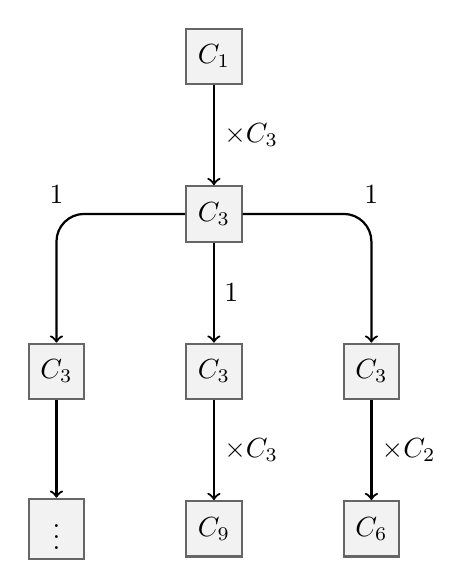
\begin{tikzpicture}[
	t/.style = {rectangle, draw=black!60, fill=black!5, thick, minimum size=20},
	r/.style = {->, thick, rounded corners=10pt}
	]
	
	%Nodes
	\node[t]	(0)		at	(0, 6)	{$C_1$};
	\node[t]	(1)		at	(0, 4)	{$C_3$};
	\node[t]	(1-l)	at	(-2, 2)	{$C_3$};
	\node[t]	(1-c)	at	(0, 2)	{$C_3$};
	\node[t]	(1-r)	at	(2, 2)	{$C_3$};
	\node[t]	(2-l)	at	(-2, 0)	{$\vdots$};
	\node[t]	(2-c)	at	(0, 0)	{$C_9$};
	\node[t]	(2-r)	at	(2, 0)	{$C_6$};
	
	
	%Lines
	\draw[r]	(0.south)	to	node[right]	{$\times C_3$}	(1.north);
	\draw[r]	(1.west)	-|	node[above]	{$1$}			(1-l.north);
	\draw[r]	(1.south)	to	node[right]	{$1$}			(1-c.north);
	\draw[r]	(1.east)	-|	node[above]	{$1$}			(1-r.north);
	\draw[r]	(1-l.south)	to								(2-l.north);
	\draw[r]	(1-c.south)	to	node[right]	{$\times C_3$}	(2-c.north);
	\draw[r]	(1-r.south)	to	node[right]	{$\times C_2$}	(2-r.north);
	
\end{tikzpicture}






\vspace{0.3in}

Как мы видим, циклические группы $C_9$ и $C_6$ находятся в дереве деления на одинаковых уровнях. Это и есть пример применения нетривиальных разложений. Давайте же тогда рассмотрим некоторые разбиения, например, дроби $\frac{34}{108}$:


\begin{align*}
	\frac{34}{108} = \frac{17}{54} = &\frac{1}{54} + \frac{8}{27} = \frac{1}{54} + \frac{2}{27} + \frac{2}{9} \\
	&\frac{1}{27} + \frac{5}{18} = \frac{1}{27} + \frac{1}{18} + \frac{2}{9} \\
	&\quad\quad\quad\quad\quad\frac{1}{27} + \frac{1}{9} + \frac{1}{6}
\end{align*}















\vspace{0.5in}

\subsection{Несколько входов}

\

Порой бывает такое, что мы имеем несколько входных конвейеров, идущих, например, с разных производств, и нам необходимо как-то перераспределить между ними ресурсы.

\

Можно пойти двумя путями: по \underline{принципу чайника}%
\footnote{Как физик заваривает чай, если чайник пустой? Наливает воду, кипитит воду, заваривает чай. \\ Как математик заваривает чай, если чайник пустой? Наливает воду, кипитит воду, заваривает чай. \\ Как физик заваривает чай, если в чайнике есть вода? Кипитит воду, заваривает чай. \\ Как математик заваривает чай, если в чайнике есть вода? Выливает воду, наливает воду, кипитит воду, заваривает чай. \\ Принцип чайника: сведи задачу к предыдущей.}
: соединить все входные конвейеры, и работать с тем, что получим; или  поиграться с отделениями в самих конвейерах. Рассматривать мы будем второй метод, так как он является обобщением первого.

\

\noindent Пример:

Входы: 4, 8, 10, 18

Выходы: 5, 8, 12, 15

\vspace{0.5in}

\begin{minipage}{0.4\textwidth}
	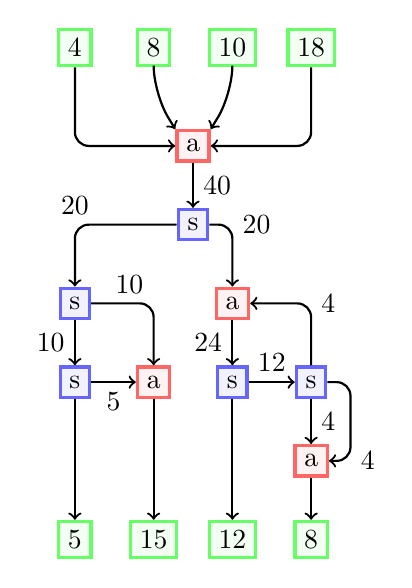
\begin{tikzpicture}[
		s/.style = {rectangle, draw=blue!60,	fill=blue!5,	very thick, minimum size=10},
		a/.style = {rectangle, draw=red!60,		fill=red!5,		very thick, minimum size=10},
		o/.style = {rectangle, draw=green!60,	fill=green!5,	very thick, minimum size=10},
		r/.style = {->, thick, rounded corners=5pt},
		b/.style = {->, thick, rounded corners=10pt}
		]
		
		% === === Nodes === ===
		\node[o]	(in1)	at	(-1, 3.25)		{$4$};	
		\node[o]	(in2)	at	(0, 3.25)		{$8$};	
		\node[o]	(in3)	at	(1, 3.25)		{$10$};	
		\node[o]	(in4)	at	(2, 3.25)		{$18$};
		\node[a]	(a0)	at	(0.5, 2)		{a};
		\node[s]	(s1)	at	(0.5, 1)		{s};
		
		\node[s]	(s2)	at	(-1, 0)			{s};
		\node[a]	(a1)	at	(1, 0)			{a};
		\node[s]	(s3-l)	at	(-1, -1)		{s};
		\node[s]	(s3-c)	at	(1, -1)			{s};
		\node[s]	(s3-r)	at	(2, -1)			{s};
		\node[a]	(a2-l)	at	(0, -1)			{a};
		\node[a]	(a2-r)	at	(2, -2)			{a};
		
		\node[o]	(out1)	at	(-1, -3)		{$5$};
		\node[o]	(out2)	at	(0, -3)			{$15$};
		\node[o]	(out3)	at	(1, -3)			{$12$};
		\node[o]	(out4)	at	(2, -3)			{$8$};
		
		
		
		% === === Lines === ===
		\draw[r]	(in1.south)		|-							(a0.west);
		\draw[r]	(in4.south)		|-							(a0.east);
		\draw[b] (in2.south) -- (0, 2.667) -- (a0.north west);
		\draw[b] (in3.south) -- (1, 2.667) -- (a0.north east);
		\draw[r]	(a0.south)		to	node[right]	{$40$}	(s1.north);
		
		\draw[r]	(s1.west)		-|	node[above]		{$20$}	(s2.north);
		\draw[r]	(s1.east)		-|	node[right]		{$20$}	(a1.north);
		\draw[r]	(s2.south)		to	node[left]		{$10$}	(s3-l.north);
		\draw[r] 	(s3-l.east) 	to 	node[below] 	{$5$} 	(a2-l.west);
		\draw[r]	(s2.east)		-|	node[above left]	{$10$}	(a2-l.north);	
		
		\draw[r]	(a1.south)		to	node[left]		{$24$}	(s3-c.north);
		\draw[r]	(s3-c.east)		to	node[above]		{$12$}	(s3-r.west);
		\draw[r]	(s3-r.north)	|-	node[right]		{$4$}	(a1.east);
		\draw[r]	(s3-r.south)	to	node[right]		{$4$}	(a2-r.north);
		\draw[r] (s3-r.east) -| (2.5, -1.5) |- node[right] {$4$} (a2-r.east);
		
		\draw[r]	(s3-l.south)	to							(out1.north);
		\draw[r]	(a2-l.south)	to							(out2.north);
		\draw[r]	(s3-c.south)	to							(out3.north);
		\draw[r]	(a2-r.south)	to							(out4.north);
		
		
	\end{tikzpicture}
\end{minipage}
\begin{minipage}{0.4\textwidth}
	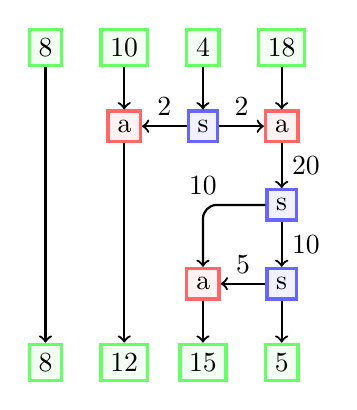
\begin{tikzpicture}[
		s/.style = {rectangle, draw=blue!60,	fill=blue!5,	very thick, minimum size=10},
		a/.style = {rectangle, draw=red!60,		fill=red!5,		very thick, minimum size=10},
		o/.style = {rectangle, draw=green!60,	fill=green!5,	very thick, minimum size=10},
		r/.style = {->, thick, rounded corners=5pt},
		b/.style = {->, thick, rounded corners=10pt}
		]
		
		% === === Nodes === ===
		\node[o]	(in1)	at	(-1, 3)		{$8$};	
		\node[o]	(in2)	at	(0, 3)		{$10$};	
		\node[o]	(in3)	at	(1, 3)		{$4$};	
		\node[o]	(in4)	at	(2, 3)		{$18$};
		
		\node[s]	(s0)	at	(1, 2)		{s};
		\node[a]	(a0-r)	at	(2, 2)		{a};
		\node[a]	(a0-l)	at	(0, 2)		{a};
		\node[s]	(s1)	at	(2, 1)		{s};
		\node[s]	(s2)	at	(2, 0)		{s};
		\node[a]	(a1)	at	(1, 0)		{a};
		
		\node[o]	(out1)	at	(-1, -1)	{$8$};	
		\node[o]	(out2)	at	(0, -1)		{$12$};	
		\node[o]	(out3)	at	(1, -1)		{$15$};	
		\node[o]	(out4)	at	(2, -1)		{$5$};
		
		
		
		% === === Lines === ===
		\draw[r] 	(in1.south)		to	(out1.north);
		\draw[r]	(in2.south)		to	(a0-l.north);
		\draw[r]	(in3.south)		to	(s0.north);
		\draw[r]	(in4.south)		to	(a0-r.north);
		\draw[r]	(a0-l.south)	to	(out2.north);
		\draw[r]	(a1.south)		to	(out3.north);
		\draw[r]	(s2.south)		to	(out4.north);
		
		\draw[r]	(s0.west)		to	node[above]	{$2$}	(a0-l.east);
		\draw[r]	(s0.east)		to	node[above]	{$2$}	(a0-r.west);
		\draw[r]	(a0-r.south)	to	node[right]	{$20$}	(s1.north);
		\draw[r]	(s1.south)		to	node[right]	{$10$}	(s2.north);
		\draw[r]	(s1.west)		-|	node[above]	{$10$}	(a1.north);
		\draw[r]	(s2.west)		to	node[above]	{$5$}	(a1.east);
		
	\end{tikzpicture}
\end{minipage}





\vspace{0.5in}

Очевидно, что вторая схема проще первой. Хотя, на самом деле, это не всегда так, и нам просто повезло. Иногда эти две схемы могут быть вообще одинаковыми (например от (10, 10, 10, 10) отделить (5, 8, 12, 15)). 

\

Однако даже так, её можно упростить: как нам уже известно, такая схема является матрицей преобразования вида:



$$
\left[
\begin{matrix}
	5 \\ 8 \\ 15 \\ 12
\end{matrix}
\right]
=
\left[
\begin{matrix}
	m_{11} & \ldots & m_{14} \\
	\vdots & \ddots & \vdots \\
	m_{41} & \ldots & m_{44}
\end{matrix}
\right]
\times
\left[
\begin{matrix}
	10 \\ 8 \\ 4 \\ 18
\end{matrix}
\right]
$$



\

\noindent И имеет решение, например:

$$
\left[
\begin{matrix}
	5 \\ 8 \\ 15 \\ 12
\end{matrix}
\right]
=
\left[
\begin{matrix}
	\frac12 & 0 & 0 & 0 \\
	0 		& 1 & 0 & 0 \\
	\frac12 & 0 & 1	& \frac13 \\
	0		& 0 & 0 & \frac23 \\
\end{matrix}
\right]
\times
\left[
\begin{matrix}
	10 \\ 8 \\ 4 \\ 18
\end{matrix}
\right]
$$






\vspace{0.5in}


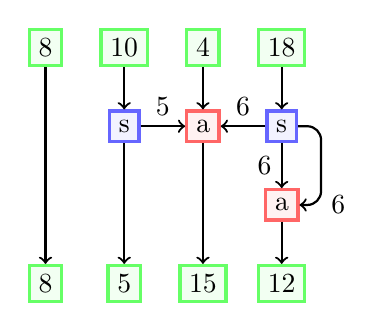
\begin{tikzpicture}[
	s/.style = {rectangle, draw=blue!60,	fill=blue!5,	very thick, minimum size=10},
	a/.style = {rectangle, draw=red!60,		fill=red!5,		very thick, minimum size=10},
	o/.style = {rectangle, draw=green!60,	fill=green!5,	very thick, minimum size=10},
	r/.style = {->, thick, rounded corners=5pt},
	b/.style = {->, thick, rounded corners=10pt}
	]
	
	% === === Nodes === ===
	\node[o]	(in1)	at	(-1, 3)	{$8$};	
	\node[o]	(in2)	at	(0, 3)	{$10$};	
	\node[o]	(in3)	at	(1, 3)	{$4$};	
	\node[o]	(in4)	at	(2, 3)	{$18$};
	
	\node[s]	(s1)	at	(0, 2)	{s};
	\node[s]	(s2)	at	(2, 2)	{s};
	\node[a]	(a1)	at	(1, 2)	{a};
	\node[a]	(a2)	at	(2, 1)	{a};
	
	\node[o]	(out1)	at	(-1, 0)	{$8$};	
	\node[o]	(out2)	at	(0, 0)	{$5$};	
	\node[o]	(out3)	at	(1, 0)	{$15$};	
	\node[o]	(out4)	at	(2, 0)	{$12$};
	
	
	
	% === === Lines === ===
	\draw[r]	(in1.south)	to	(out1.north);
	\draw[r]	(in2.south)	to	(s1.north);
	\draw[r]	(s1.south)	to	(out2.north);
	\draw[r]	(s1.east)	to	node[above]	{$5$}	(a1.west);
	\draw[r]	(in3.south)	to	(a1.north);
	\draw[r]	(in4.south)	to	(s2.north);
	\draw[r]	(s2.west)	to	node[above]	{$6$}	(a1.east);
	\draw[r]	(a1.south)	to	(out3.north);
	\draw[r]	(s2.south)	to	node[left]	{$6$}	(a2.north);
	\draw[r]	(s2.east)	-|	(2.5, 1.5)	|-	node[right]	{$6$}	(a2.east);
	\draw[r]	(a2.south)	to	(out4.north);
	
\end{tikzpicture}



\vspace{0.5in}

Таким образом, мы получили самую простую версию схемы перераспределения ресурсов между несколькими входами и выходами.






























































\vspace{1in}

\section{Решение}

\

\noindent Любую стандартную долю можно представить, как сумму некоторого количества других стандартных дробей:

$$\forall \ \frac{a}{s} \ : \ \exists \ n \in \mathbb{N}, A = \{a_i\}, S = \{s_i\} \ | \ \frac{a}{s} = \sum_{i=1}^n \frac{a_i}{s_i}$$

\

\noindent "Элементарными" назовём несократимые стандартные дроби, для которых $n=1$, т.е.: 

$\nexists \ a_i \le a \ | \ \text{gcd}(a_i, s) \ne 1$

\

\noindent Для дроби $\frac{a}{b}$ "решением" назовём%
\footnote{под "-" подразумеваем его определение через рекурсию}
$A_b^a = O_b^a - R_b$, где:


\begin{itemize}
	\item $s = s(b)$ -- ближайшее большее стандартное к $b$
	
	\item $O_b^a = O_{s}^a = \sum_{i=1}^n \frac{a_i}{s_i}$
	
	\item $R_b = O_{s}^{s-b}$
\end{itemize}

\

\noindent Тогда задача сводится к изучению получения оптимальных $S(b)$, $O_s^a$ и $R_b$.





\vspace{0.5in}

\noindent Код на C\# для реализации поиска наименьшего $s(b)$ для множества $\mathbb{T} = \{ 2, 3 \}$:

\newpage

\begin{lstlisting}[title={C\#}, language={[Sharp]C}]
public static int hig_closest(int number, int x = 0, int y = 0, int branch = 1)
{
	int answer = -1;
	int num = Convert.ToInt32(Math.Pow(2, x) * Math.Pow(3, y));
	
	if (num >= number) { answer = num; }
	else
	{
		List<int> answers = new List<int>();
		
		answers.Add(hig_closest(number, x + 1, y, 0));
		if (branch == 1) 
		{ answers.Add(hig_closest(number, x, y + 1, 1)); }
		
		answer = answers.Min();
	}
	
	return answer;
}
\end{lstlisting}



\vspace{0.5in}

\noindent Он реализует следующее дерево поиска (пример для $b=31$):

\vspace{0.35in}

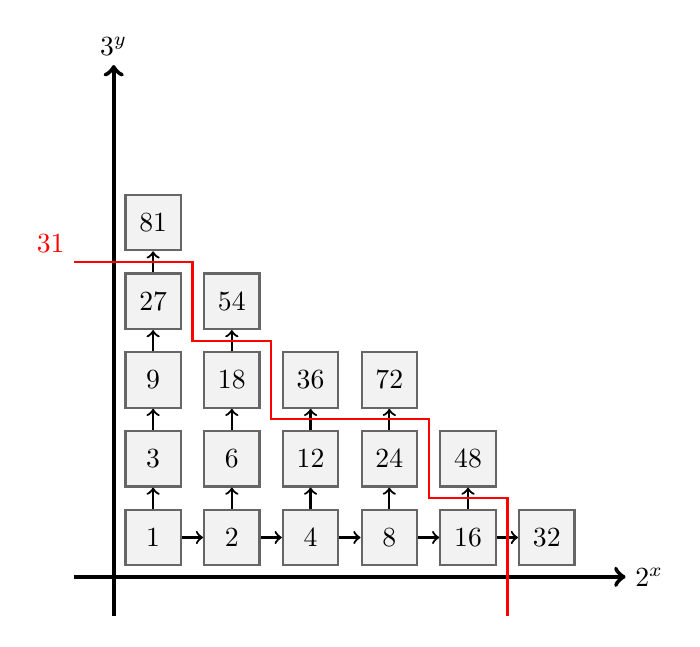
\begin{tikzpicture}[
	t/.style = {rectangle, draw=black!60, fill=black!5, thick, minimum size=20},
	r/.style = {->, thick, rounded corners=10pt}
	]
	
	% === === === Nodes === === ===
	\node[t]	(0-0)	at	(0, 0)	{1};
	\node[t]	(1-0)	at	(1, 0)	{2};
	\node[t]	(2-0)	at	(2, 0)	{4};
	\node[t]	(3-0)	at	(3, 0)	{8};
	\node[t]	(4-0)	at	(4, 0)	{16};
	\node[t]	(5-0)	at	(5, 0)	{32};
	
	\node[t]	(0-1)	at	(0, 1)	{3};
	\node[t]	(1-1)	at	(1, 1)	{6};
	\node[t]	(2-1)	at	(2, 1)	{12};
	\node[t]	(3-1)	at	(3, 1)	{24};
	\node[t]	(4-1)	at	(4, 1)	{48};
	
	\node[t]	(0-2)	at	(0, 2)	{9};
	\node[t]	(1-2)	at	(1, 2)	{18};
	\node[t]	(2-2)	at	(2, 2)	{36};
	\node[t]	(3-2)	at	(3, 2)	{72};
	
	\node[t]	(0-3)	at	(0, 3)	{27};
	\node[t]	(1-3)	at	(1, 3)	{54};
	
	\node[t]	(0-4)	at	(0, 4)	{81};
	
	
	
	% === === === Axis === === ===
	\draw[->, ultra thick]	(-1, -0.5) to (6, -0.5);
	\node[right] (x) at (6, -0.5) {$2^x$};
	\draw[->, ultra thick]	(-0.5, -1) to (-0.5, 6);
	\node[above] (y) at (-0.5, 6) {$3^y$};
	
	
	
	% === === === Lines === === ===
	\draw[r] (0-0.east) to (1-0.west);
	\draw[r] (1-0.east) to (2-0.west);
	\draw[r] (2-0.east) to (3-0.west);
	\draw[r] (3-0.east) to (4-0.west);
	\draw[r] (4-0.east) to (5-0.west);
	
	\draw[r] (0-0.north) to (0-1.south);
	\draw[r] (0-1.north) to (0-2.south);
	\draw[r] (0-2.north) to (0-3.south);
	\draw[r] (0-3.north) to (0-4.south);
	
	\draw[r] (1-0.north) to (1-1.south);
	\draw[r] (1-1.north) to (1-2.south);
	\draw[r] (1-2.north) to (1-3.south);
	
	\draw[r] (2-0.north) to (2-1.south);
	\draw[r] (2-1.north) to (2-2.south);
	
	\draw[r] (3-0.north) to (3-1.south);
	\draw[r] (3-1.north) to (3-2.south);
	
	\draw[r] (4-0.north) to (4-1.south);
	
	\draw[thick, red] (-1, 3.5) -- (0.5, 3.5) -- (0.5, 2.5) -- (1.5, 2.5) -- (1.5, 1.5) -- (3.5, 1.5) -- (3.5, 0.5) -- (4.5, 0.5) -- (4.5, -1);
	\node[above left, color=red] (31) at (-1, 3.5) {31};
	
	
\end{tikzpicture}





\vspace{0.35in}

\noindent Нетрудно модифицировать данный алгоритм для произвольных $\mathbb{T}$:

\vspace{0.2in}

\begin{lstlisting}[title={Python}, language={Python}]
def hig_closest(target, powers, branch=max(T)):
	answer = -1
	num = 1
	for i in range(0, T.len()):
		num *= T[i]**powers[i]
	
	if num >= target: return num
	
	answers = []
	for i in T:
		if i <= branch>:
			answers.append(hig_closest(target, powers.increace(i), i))
	
	answer = min(answers)
	
	return answer
\end{lstlisting}

\vspace{0.5in}




Вот нашли мы $s(b)$, а как теперь искать $O_s^a$? Ответ прост: брутфорс. Требуется перебрать все возможные способы разбиения числа $a$ на суммы всевозможных натуральных%
\footnote{Вцелом, можно и не натуральных, а просто рациональных: $\frac23 = \frac{1.5}3 + \frac{0.5}3 = \frac12 + \frac16$ -- такое разбиение вполне подойдёт для $\mathbb{T} = \{2, 6\}$. Однако, такой алгоритм слишком сложен, ведь перебирать придётся \textbf{значительно} больше вариантов}
чисел, после чего соответствующие дроби (если это возможно) мы сокрращаем дроби, а затем объединяем все дроби с одинаковыми знаменателями. Для каждого отдельного знаменателя $s_i = \prod_{j=0}^n t_j^{a_j}$ должно быть выполненно: $s_i < t_j \ \forall j$

% \
%
% !!!!! Нужно раздеять не до единиц, а только на: !!!!!
% $$a = \sum_{a_i < b \ \forall b \in \mathbb{T}} a_i$$

\

\noindent Алгоритм для поиска одного варианта разбиения:

\

\begin{lstlisting}[title={Python}, language={Python}]
def spliter(numerator, denominator):
	s = hig_closest(denominator)
	reduce_coef = gcd(s, numerator)
	numerator //= reduce_coef
	denominator = s // reduce_coef
	
	s = low_closest(numerator, denominator)
	
	if s == numerator:
		return [[numerator, denominator]]
	
	else:
		cdg1 = gcd(numerator-s, denominator)
		gcd2 = gcd(s, denominator)
		d_parts = [
			[(numerator-s)//gcd1, denominator//gcd1], 
			[s//gcd2, denominator//gdc2]
		]
	
	while 1:
		memory = []
	
		for fractions in d_parts:
			x, y = fractions[0], fractions[1]
			s = low_closest(x, y)
		
			if p != x:
				gcd1 = gcd(x-s, y)
				gcd2 = gcd(s, y)
				memory.append([(x-s)//gcd1, y//gcd1])
				memory.append([s//gcd2, y//gcd2])
			
			else: memory.append(fractions)
		
		if len(d_parts) == len(memory): break
		else: d_parts = memory[0::]
		
	return d_parts[0::]
\end{lstlisting}



\vspace{0.5in}

\noindent Полноценный алгоритм на C\# приведён в satisfactory\_conveyor\_calc.sln

































































\newpage

\section{Построение схемы}

\subsection{Степенное дерево}

\

Самый простой способ: если известно решение $A_b^a = O_b^a - R_b$ -- то можно просто в лоб реализовать дерево на $s$ листьев, $s-b$ из них вернуть в начало, $a$ соединить, и отправить на выход; а оставшиеся $b-a$ тоже соединить, и тоже на выход.

\vspace{0.5in}

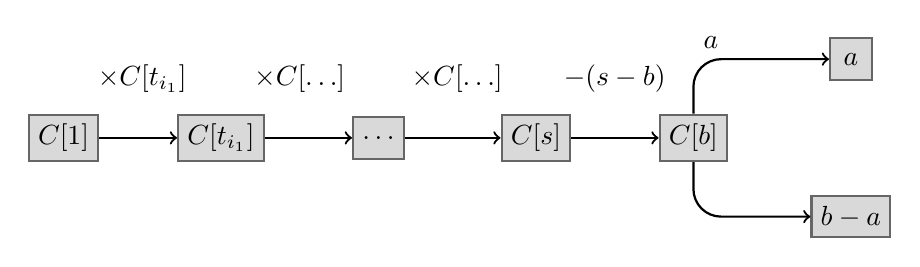
\begin{tikzpicture}[
	t/.style = {rectangle, draw=black!60, fill=black!15, thick, minimum size=15},
	r/.style = {->, thick, rounded corners=10pt}
	]
	
	%Nodes
	\node[t]	(1)		at	(-4, 0)		{$C[1]$};
	\node[t]	(2)		at	(-2, 0)		{$C[t_{i_1}]$};
	\node[t]	(e)		at	(0, 0)		{$\ldots$};
	\node[t]	(s)		at	(2, 0)		{$C[s]$};
	\node[t]	(b)		at	(4, 0)		{$C[b]$};
	
	\node		(t1)	at	(-3, 0.75)	{$\times C[t_{i_1}]$};
	\node		(t2)	at	(-1, 0.75)	{$\times C[\ldots]$};
	\node		(t3)	at	(1, 0.75)	{$\times C[\ldots]$};
	\node		(t4)	at	(3, 0.75)	{$- (s-b)$};

	\node[t]	(A)		at	(6, 1)		{$a$};
	\node[t]	(B)		at	(6, -1)		{$b-a$};
	
	
	
	%Lines
	\draw[r]	(1.east)	to	(2.west);
	\draw[r]	(2.east)	to	(e.west);
	\draw[r]	(e.east)	to	(s.west);
	\draw[r]	(s.east)	to	(b.west);
	\draw[r]	(b.north)	|-	node[above right]	{$a$}	(A.west);
	\draw[r]	(b.south)	|-	(B.west);
\end{tikzpicture}





\vspace{0.5in}

\noindent Аналогично можно реализовать схему для отделения $a_1$, $a_2$, ..., $a_n$ от $b$:

\vspace{0.5in}

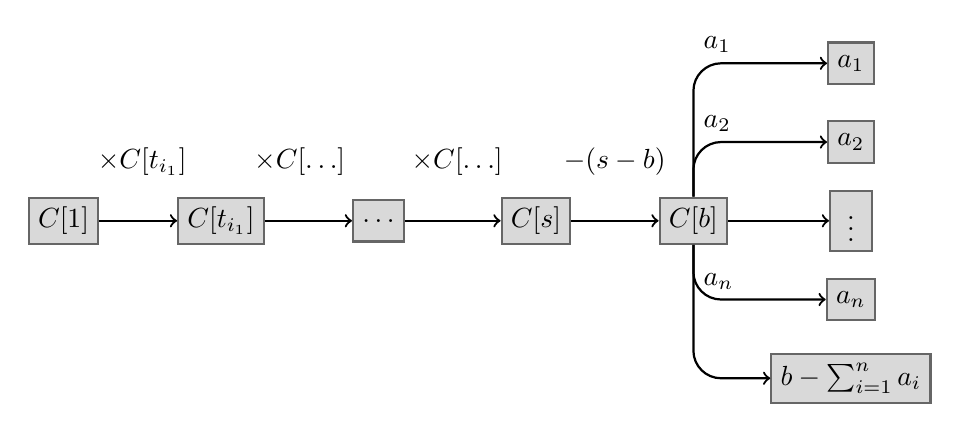
\begin{tikzpicture}[
	t/.style = {rectangle, draw=black!60, fill=black!15, thick, minimum size=15},
	r/.style = {->, thick, rounded corners=10pt}
	]
	
	%Nodes
	\node[t]	(1)		at	(-4, 0)		{$C[1]$};
	\node[t]	(2)		at	(-2, 0)		{$C[t_{i_1}]$};
	\node[t]	(e)		at	(0, 0)		{$\ldots$};
	\node[t]	(s)		at	(2, 0)		{$C[s]$};
	\node[t]	(b)		at	(4, 0)		{$C[b]$};
	
	\node		(t1)	at	(-3, 0.75)	{$\times C[t_{i_1}]$};
	\node		(t2)	at	(-1, 0.75)	{$\times C[\ldots]$};
	\node		(t3)	at	(1, 0.75)	{$\times C[\ldots]$};
	\node		(t4)	at	(3, 0.75)	{$- (s-b)$};
	
	\node[t]	(A1)	at	(6, 2)		{$a_1$};
	\node[t]	(A2)	at	(6, 1)		{$a_2$};
	\node[t]	(Ae)	at	(6, 0)		{$\vdots$};
	\node[t]	(An)	at	(6, -1)		{$a_n$};
	\node[t]	(B)		at	(6, -2)		{$b - \sum_{i=1}^n a_i$};
	
	
	
	%Lines
	\draw[r]	(1.east)	to	(2.west);
	\draw[r]	(2.east)	to	(e.west);
	\draw[r]	(e.east)	to	(s.west);
	\draw[r]	(s.east)	to	(b.west);
	\draw[r]	(b.north)	|-	node[above right]	{$a_1$}	(A1.west);
	\draw[r]	(b.north)	|-	node[above right]	{$a_2$}	(A2.west);
	\draw[r]	(b.east)	to	(Ae.west);
	\draw[r]	(b.south)	|-	node[above right]	{$a_n$}	(An.west);
	\draw[r]	(b.south)	|-	(B.west);
\end{tikzpicture}




\vspace{0.5in}

\noindent Однако, если $s = \prod_{i=1}^k t_{j_i}^{\alpha_i}$ -- то такое решение займёт:

$$
\left( 
k 
\ ; \ 
\prod_{i=1}^k t_{j_i}^{\alpha_i} 
\right)
$$


\noindent Если требуется показать суть зависимости -- то масштабы можно редуцировать до: 

$$\left(x; e^x\right)$$

\

В общем: площадь растёт экспоненциально в зависимости от сложности схемы, что очень неудобно, особенно для сложных базисов.















\newpage

\subsection{Ёлочка}

\

Однако, как мы уже знаем, схемы предыдущего вида можно сократить. первым уровнем аппроксимации упрощения является "ёлочка". Рассмотрим ситуацию $S(b) = b$:

$$\frac{a}{b} = \sum_{i=1}^n \frac{a_i}{s_i} 
\quad \quad
s_i = s_{i-1} \cdot \prod_{j=1}^{k_i} t_{ij}^{\alpha_{ij}}
\quad \quad
s_0 = 1
\quad \quad
a_i < \text{min}(t_{ij})
$$

\

\noindent Пускай, каждый $t_i$ повторяется ровно $\alpha_i$ раз внутри одного $s_i$. Будем реализовывать $s_i$ один за другим:




\vspace{0.5in}

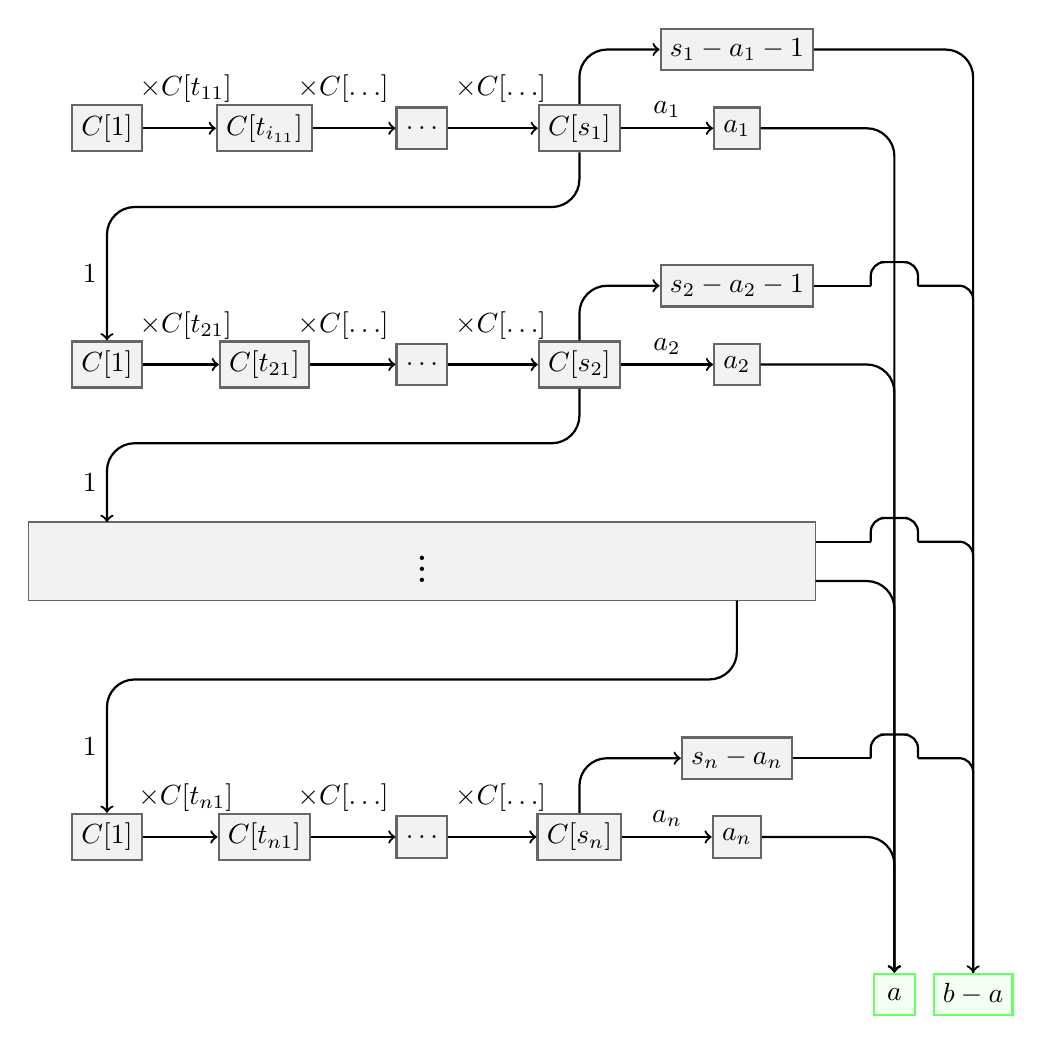
\begin{tikzpicture}[
	o/.style = {rectangle, draw=green!60,	fill=green!5,	thick, minimum size=15},
	t/.style = {rectangle, draw=black!60, 	fill=black!5, 	thick, minimum size=15},
	r/.style = {->, thick, rounded corners=10pt}
	]
	
	% ===== ===== ===== ===== =====
	
	% Nodes
	\node[t]	(11)	at	(-4, 0)		{$C[1]$};
	\node[t]	(12)	at	(-2, 0)		{$C[t_{i_{11}}]$};
	\node[t]	(1e)	at	(0, 0)		{$\ldots$};
	\node[t]	(1s)	at	(2, 0)		{$C[s_1]$};
	
	\node		(1t1)	at	(-3, 0.5)	{$\times C[t_{11}]$};
	\node		(1t2)	at	(-1, 0.5)	{$\times C[\ldots]$};
	\node		(1t3)	at	(1, 0.5)	{$\times C[\ldots]$};
	
	\node[t]	(1B)	at	(4, 1)		{$s_1-a_1-1$};
	\node[t]	(1A)	at	(4, 0)		{$a_1$};
	
	
	
	% Lines
	\draw[r]	(11.east)	to	(12.west);
	\draw[r]	(12.east)	to	(1e.west);
	\draw[r]	(1e.east)	to	(1s.west);
	\draw[r]	(1s.north)	|-	(1B.west);
	\draw[r]	(1s.east)	to	node[above]	{$a_1$}	(1A.west);
	
	
	
	% ===== ===== ===== ===== =====
	
	% Nodes
	\node[t]	(21)	at	(-4, -3)	{$C[1]$};
	\draw[r] (1s.south) |- (-4, -1) to node[left] {$1$} (21.north);
	
	\node[t]	(22)	at	(-2, -3)	{$C[t_{21}]$};
	\node[t]	(2e)	at	(0, -3)		{$\ldots$};
	\node[t]	(2s)	at	(2, -3)		{$C[s_2]$};
	
	\node		(2t1)	at	(-3, -2.5)	{$\times C[t_{21}]$};
	\node		(2t2)	at	(-1, -2.5)	{$\times C[\ldots]$};
	\node		(2t3)	at	(1, -2.5)	{$\times C[\ldots]$};
	
	\node[t]	(2B)	at	(4, -2)		{$s_2-a_2-1$};
	\node[t]	(2A)	at	(4, -3)		{$a_2$};
	
	
	
	% Lines
	\draw[r]	(21.east)	to	(22.west);
	\draw[r]	(22.east)	to	(2e.west);
	\draw[r]	(2e.east)	to	(2s.west);
	\draw[r]	(2s.north)	|-	(2B.west);
	\draw[r]	(2s.east)	to	node[above]	{$a_2$}	(2A.west);
	
	
	
	% ===== ===== ===== ===== ===== 
	\draw[draw=black!60, fill=black!5] (-5, -5) rectangle node {$\textbf{\vdots}$} (5, -6);
	\draw[r] (2s.south) |- (-4, -4) to node[left] {$1$} (-4, -5);
	
	
	
	% ===== ===== ===== ===== =====
	
	% Nodes
	\node[t]	(n1)	at	(-4, -9)	{$C[1]$};
	\draw[r] (4, -6) |- (-4, -7) to node[left] {$1$} (n1.north);
	
	\node[t]	(n2)	at	(-2, -9)	{$C[t_{n1}]$};
	\node[t]	(ne)	at	(0, -9)		{$\ldots$};
	\node[t]	(ns)	at	(2, -9)		{$C[s_n]$};
	
	\node		(nt1)	at	(-3, -8.5)	{$\times C[t_{n1}]$};
	\node		(nt2)	at	(-1, -8.5)	{$\times C[\ldots]$};
	\node		(nt3)	at	(1, -8.5)	{$\times C[\ldots]$};
	
	\node[t]	(nB)	at	(4, -8)		{$s_n-a_n$};
	\node[t]	(nA)	at	(4, -9)		{$a_n$};
	
	
	
	% Lines
	\draw[r]	(n1.east)	to	(n2.west);
	\draw[r]	(n2.east)	to	(ne.west);
	\draw[r]	(ne.east)	to	(ns.west);
	\draw[r]	(ns.north)	|-	(nB.west);
	\draw[r]	(ns.east)	to	node[above]	{$a_n$}	(nA.west);
	
	
	
	% ===== ===== ===== ===== =====
	
	% Nodes
	\node[o]	(out1)	at	(6, -11)	{$a$};
	\node[o]	(out2)	at	(7, -11)	{$b-a$};
	
	% Lines
	\draw[r]	(1A.east)	-|	(out1.north);
	\draw[r]	(2A.east)	-|	(out1.north);
	\draw[r]	(5, -5.75)	-|	(out1.north);
	\draw[r]	(nA.east)	-|	(out1.north);
	
	\draw[r]	(1B.east)	-|	(out2.north);
	
	\draw[thick] (2B.east) to (5.7, -2);
	\draw[thick, rounded corners=5pt] (5.7, -2) |- (6, -1.7) -| (6.3, -2);
	\draw[thick, rounded corners=5pt] (6.3, -2) -| (out2.north);
	
	\draw[thick] (5, -5.25) to (5.7, -5.25);
	\draw[thick, rounded corners=5pt] (5.7, -5.25) |- (6, -4.95) -| (6.3, -5.25);
	\draw[thick, rounded corners=5pt] (6.3, -5.25) -| (out2.north);
	
	\draw[thick] (nB.east) to (5.7, -8);
	\draw[thick, rounded corners=5pt] (5.7, -8) |- (6, -7.7) -| (6.3, -8);
	\draw[thick, rounded corners=5pt] (6.3, -8) -| (out2.north);
	
\end{tikzpicture}




\vspace{0.5in}

Казалось бы, почему "ёлочка", если это "змейка" какая-то? Дело в том, что следует рассмотреть граф, а не алгебраическую схему. Рассмотрим же возможный вид контуров графа:





\vspace{0.5in}

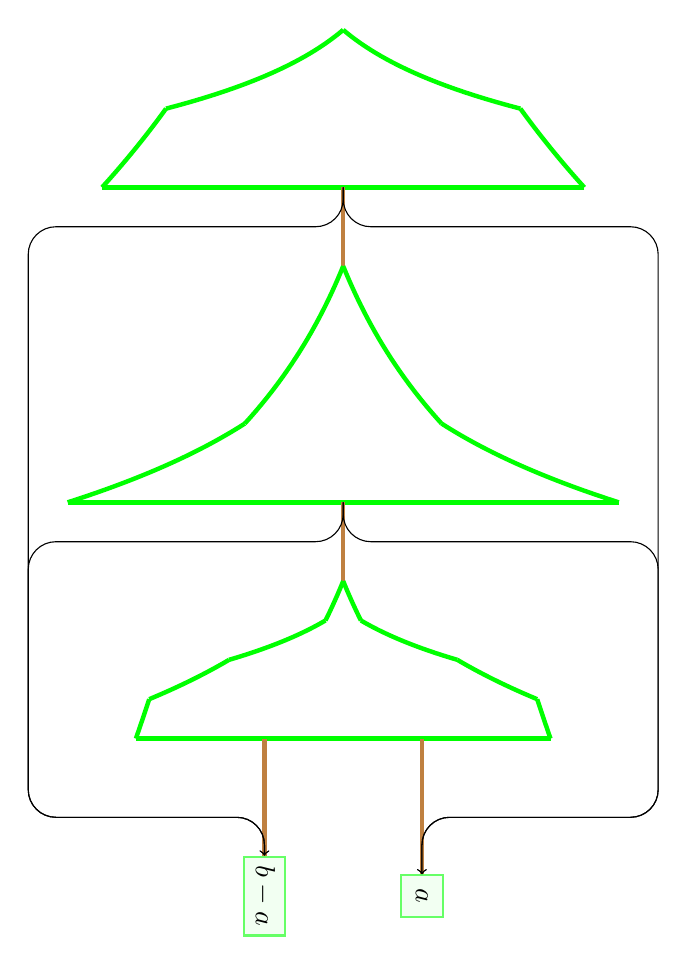
\begin{tikzpicture}[
	rotate=-90,
	o/.style = {rectangle, draw=green!60,	fill=green!5,	thick, minimum size=15},
	r/.style = {->, thin, rounded corners=10pt},
	b/.style = {ultra thick, rounded corners=10pt},
	g/.style = {ultra thick, green}
	]
	
	\begin{axis}[clip = false, 
		hide axis, 
		x=1cm, y=1cm,
		]
		
		\addplot[domain=0:1, g] {3.25^x-1};
		\addplot[domain=1:2, g] {1.25^(x-1)*3.25-1};
		\addplot[domain=0:1, g] {-3.25^x+1};
		\addplot[domain=1:2, g] {-1.25^(x-1)*3.25+1};
		
		\draw[b, green] (axis cs: 2, 3.0625) -- (axis cs:2, -3.0625);
		\draw[b, brown] (axis cs: 2, 0) -- (axis cs: 3, 0);
		
		
		
		\addplot[domain=3:5, g] {1.5^(x-3)-1};
		\addplot[domain=5:6, g] {2^(x-5)*2.25-1};
		\addplot[domain=3:5, g] {-1.5^(x-3)+1};
		\addplot[domain=5:6, g] {-2^(x-5)*2.25+1};
		
		\draw[b, green] (axis cs: 6, 3.5) -- (axis cs:6, -3.5);
		\draw[b, brown] (axis cs: 6, 0) -- (axis cs: 7, 0);
		
		\addplot[domain=7:7.5, g] {1.5^(x-7)-1};
		\addplot[domain=7.5:8, g] {4^(x-7.5)*1.5^0.5-1};
		\addplot[domain=8:8.5, g] {2^(x-8)*1.5^0.5*4^0.5-1};
		\addplot[domain=8.5:9, g] {1.1^(x-8.5)*1.5^0.5*4^0.5*2^0.5-1};
		\addplot[domain=7:7.5, g] {-1.5^(x-7)+1};
		\addplot[domain=7.5:8, g] {-4^(x-7.5)*1.5^0.5+1};
		\addplot[domain=8:8.5, g] {-2^(x-8)*1.5^0.5*4^0.5+1};
		\addplot[domain=8.5:9, g] {-1.1^(x-8.5)*1.5^0.5*4^0.5*2^0.5+1};
		
		\draw[b, green] (axis cs: 9, 2.6332) -- (axis cs: 9, -2.6332);
		
		
		
		\node[o]	(out1)	at	(axis cs: 11, 1)	{$a$};
		\node[o]	(out2)	at	(axis cs: 11, -1)	{$b-a$};
		
		
		
		\draw[b, brown] (axis cs: 9, 1)  to (out1.west);
		\draw[b, brown] (axis cs: 9, -1) to (out2.west);
		\draw[r] (axis cs: 2, 0) -| (axis cs: 2.5, 4)  -- (axis cs: 10, 4)  |- (out1.west);
		\draw[r] (axis cs: 2, 0) -| (axis cs: 2.5, -4) -- (axis cs: 10, -4) |- (out2.west);
		\draw[r] (axis cs: 6, 0) -| (axis cs: 6.5, 4)  -- (axis cs: 10, 4)  |- (out1.west);
		\draw[r] (axis cs: 6, 0) -| (axis cs: 6.5, -4) -- (axis cs: 10, -4) |- (out2.west);
		
		
	\end{axis}
\end{tikzpicture}




\vspace{0.5in}

И действительно: теперь проглядываются "ствол", и крона, которая сначала нарастает-нарастает-нарастает, а затем резко убывает в ноль, и оголяет ствол. И картинка становится похожа на ёлку. 

\

\noindent Так же, такой тип схем занимает меньше места, чем простое дерево: 

$$ 
\sum_{i=1}^{n} 
\left( 
k_i
\ ; \ 
\prod_{j=1}^{k_i} t_{ij}^{\alpha_{ij}} 
\right)
$$

\

\noindent Или, если очень грубо округлять:

$$
\left(
k
\ ; \ 
\text{max}\left(
	\prod_{j=1}^{k_i} t_{ij}^{\alpha_{ij}}
	\right)
\right)
$$

\

Работает это за счёт того, что мы поочерёдно реализуем небольшие степенные деревья, и предварительно успеваем их обрезать, предотвращая экспоненциальный взрыв. Суть та же, что и у линзы френеля. Таким образом, редуцировать размер можно до: 

$$\left(x, e^{x/k}\right)$$

\

Так же, такую схему очень удобно реализовывать в 3D играх: каждую отдельную крону можно выносить на отдельный этаж, что позволит сильно сэкономить вплощади ценой высоты. Однако нарисовать общую схему под произвольное число выходов будет сложно, хотя реализовывать отдельно ничто не запрещает.





















\vspace{1in}

\subsection{Палочка}

\

При всём при этом, можно сократить даже ёлочку: раз у нас $a_i < \text{min}(t_{ij})$ -- то никто нам не гарантирует, что это верно идля остатка -- так что остаток мы и будем скращать. Выберем любое $t_{ij} \ | \ a_i < t_{ij}$, и поставим его в конец очереди для $s_i$:




\vspace{0.5in}

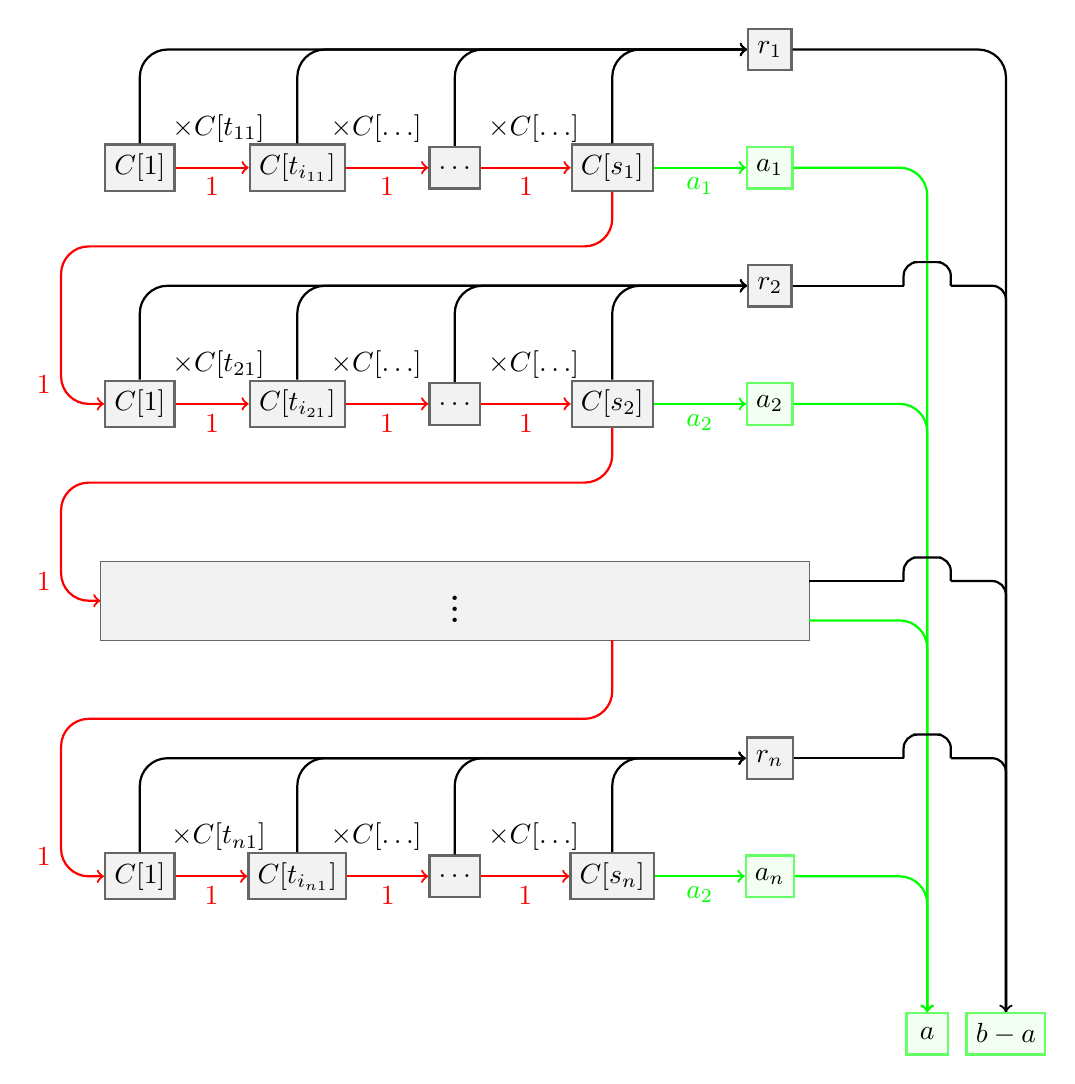
\begin{tikzpicture}[
	o/.style = {rectangle, draw=green!60,	fill=green!5,	thick, minimum size=15},
	t/.style = {rectangle, draw=black!60, 	fill=black!5, 	thick, minimum size=15},
	g/.style = {rectangle, draw=green!60, 	fill=green!5, 	thick, minimum size=15},
	r/.style = {->, thick, rounded corners=10pt}
	]
	
	% ===== ===== ===== ===== =====
	
	% Nodes
	\node[t]	(11)	at	(-4, 0)		{$C[1]$};
	\node[t]	(12)	at	(-2, 0)		{$C[t_{i_{11}}]$};
	\node[t]	(1e)	at	(0, 0)		{$\ldots$};
	\node[t]	(1s)	at	(2, 0)		{$C[s_1]$};
	
	\node		(1t1)	at	(-3, 0.5)	{$\times C[t_{11}]$};
	\node		(1t2)	at	(-1, 0.5)	{$\times C[\ldots]$};
	\node		(1t3)	at	(1, 0.5)	{$\times C[\ldots]$};
	
	\node[g]	(1A)	at	(4, 0)		{$a_1$};
	\node[t]	(1B)	at	(4, 1.5)	{$r_1$};
	
	
	
	% Lines
	\draw[r, red]	(11.east)	to	node[below]	{$1$}	(12.west);
	\draw[r, red]	(12.east)	to	node[below]	{$1$}	(1e.west);
	\draw[r, red]	(1e.east)	to	node[below]	{$1$}	(1s.west);
	\draw[r, green]	(1s.east)	to	node[below]	{$a_1$}	(1A.west);
	\draw[r]	(11.north)	|-	(1B.west);
	\draw[r]	(12.north)	|-	(1B.west);
	\draw[r]	(1e.north)	|-	(1B.west);
	\draw[r]	(1s.north)	|-	(1B.west);
	
	
	
	
	
	% ===== ===== ===== ===== =====
	
	% Nodes
	\node[t]	(21)	at	(-4, -3)	{$C[1]$};
	\draw[r, red] (1s.south) |- (-5, -1) |- node[above left] {$1$} (21.west);
	
	\node[t]	(22)	at	(-2, -3)	{$C[t_{i_{21}}]$};
	\node[t]	(2e)	at	(0, -3)		{$\ldots$};
	\node[t]	(2s)	at	(2, -3)		{$C[s_2]$};
	
	\node		(2t1)	at	(-3, -2.5)	{$\times C[t_{21}]$};
	\node		(2t2)	at	(-1, -2.5)	{$\times C[\ldots]$};
	\node		(2t3)	at	(1, -2.5)	{$\times C[\ldots]$};
	
	\node[g]	(2A)	at	(4, -3)		{$a_2$};
	\node[t]	(2B)	at	(4, -1.5)	{$r_2$};
	
	
	
	% Lines
	\draw[r, red]	(21.east)	to	node[below]	{$1$}	(22.west);
	\draw[r, red]	(22.east)	to	node[below]	{$1$}	(2e.west);
	\draw[r, red]	(2e.east)	to	node[below]	{$1$}	(2s.west);
	\draw[r, green]	(2s.east)	to	node[below]	{$a_2$}	(2A.west);
	\draw[r]	(21.north)	|-	(2B.west);
	\draw[r]	(22.north)	|-	(2B.west);
	\draw[r]	(2e.north)	|-	(2B.west);
	\draw[r]	(2s.north)	|-	(2B.west);
	
	
	
	
	
	% ===== ===== ===== ===== =====
	
	\draw[draw=black!60, fill=black!5] (-4.5, -5) rectangle node {$\textbf{\vdots}$} (4.5, -6);
	\draw[r, red] (2s.south) |- (-5, -4) |- node[above left] {$1$} (-4.5, -5.5);
	
	
	
	
	
	% ===== ===== ===== ===== =====
	
	% Nodes
	\node[t]	(n1)	at	(-4, -9)	{$C[1]$};
	\draw[r, red] (2, -6) |- (-5, -7) |- node[above left] {$1$} (n1.west);
	
	\node[t]	(n2)	at	(-2, -9)	{$C[t_{i_{n1}}]$};
	\node[t]	(ne)	at	(0, -9)		{$\ldots$};
	\node[t]	(ns)	at	(2, -9)		{$C[s_n]$};
	
	\node		(nt1)	at	(-3, -8.5)	{$\times C[t_{n1}]$};
	\node		(nt2)	at	(-1, -8.5)	{$\times C[\ldots]$};
	\node		(nt3)	at	(1, -8.5)	{$\times C[\ldots]$};
	
	\node[g]	(nA)	at	(4, -9)		{$a_n$};
	\node[t]	(nB)	at	(4, -7.5)	{$r_n$};
	
	
	
	% Lines
	\draw[r, red]	(n1.east)	to	node[below]	{$1$}	(n2.west);
	\draw[r, red]	(n2.east)	to	node[below]	{$1$}	(ne.west);
	\draw[r, red]	(ne.east)	to	node[below]	{$1$}	(ns.west);
	\draw[r, green]	(ns.east)	to	node[below]	{$a_2$}	(nA.west);
	\draw[r]	(n1.north)	|-	(nB.west);
	\draw[r]	(n2.north)	|-	(nB.west);
	\draw[r]	(ne.north)	|-	(nB.west);
	\draw[r]	(ns.north)	|-	(nB.west);
	
	
	
	
	
	% ===== ===== ===== ===== =====
	
	% Nodes
	\node[o]	(out1)	at	(6, -11)	{$a$};
	\node[o]	(out2)	at	(7, -11)	{$b-a$};
	
	% Lines
	\draw[r, green]	(1A.east)	-|	(out1.north);
	\draw[r, green]	(2A.east)	-|	(out1.north);
	\draw[r, green]	(4.5, -5.75)-|	(out1.north);
	\draw[r, green]	(nA.east)	-|	(out1.north);
	
	\draw[r]	(1B.east)	-|	(out2.north);
	
	\draw[thick] (2B.east) to (5.7, -1.5);
	\draw[thick, rounded corners=5pt] (5.7, -1.5) |- (6, -1.2) -| (6.3, -1.5);
	\draw[thick, rounded corners=5pt] (6.3, -1.5) -| (out2.north);
	
	\draw[thick] (4.5, -5.25) to (5.7, -5.25);
	\draw[thick, rounded corners=5pt] (5.7, -5.25) |- (6, -4.95) -| (6.3, -5.25);
	\draw[thick, rounded corners=5pt] (6.3, -5.25) -| (out2.north);
	
	\draw[thick] (nB.east) to (5.7, -7.5);
	\draw[thick, rounded corners=5pt] (5.7, -7.5) |- (6, -7.2) -| (6.3, -7.5);
	\draw[thick, rounded corners=5pt] (6.3, -7.5) -| (out2.north);
	
\end{tikzpicture}

\vspace{0.5in}




Забавно, что площадь схем уменьшается, то есть, казалось бы, схемы -- упрощаются -- а наше алгебраическое отоброжение только усложняется... Всё по тому, что увеличивается концентрация решений, а стало быть -- и сложность. Собственно, площадь, занимаемая палочными схемами элементарна:

$$
\left(
k
\ ; \
2
\right)
$$

\

Вау! Линейная площадь! А была ведь экспоненциальная! В чём же подвох? А подвох в том, что данная схема абсолютно не масштабируема. Такие схемы можно реализовывать \textbf{только} для отделения одной величины в случае $S(b) = b$. Если $S(b) \ne b$ -- То палочковую схему построить невозможно... По крайней мере в том виде, что подан в схеме: если повезёт -- придётся избирательно выбирать порядок сплиттеров, а затем избирательно от них забирать конвейеры для возврата. А возможно придётся даже вести несколько параллельных линий, возможно даже с разными порядками действий, или вообще разными сплиттерами впринципе. Если же требуется отделить несколько значений -- то предсказать уже невозможно ничего.















































































































































